%&mybook
%\documentclass{myarticle}

\usetikzlibrary{external,through,intersections}
% Tikz options
\tikzstyle{dashdot}=[dash pattern=on .8pt off 3pt on 4pt off 3pt]
\tikzstyle{edge1}=[red,dashed]
\tikzstyle{edge2}=[blue,dotted]
\tikzstyle{edge3}=[green,dashdot]
\tikzstyle{every node}+=[inner sep=0.5mm,minimum size=2.00mm,node distance=3em,thick]
\tikzstyle{every edge}+=[thick]
\tikzstyle{every arc}+=[thick]
\tikzstyle{every path}+=[thick]
\usetikzlibrary{svg.path,calc,decorations.pathreplacing,positioning,backgrounds}
\newdimen\XCoord
\newdimen\YCoord
\newcommand*{\ExtractCoordinate}[1]{\path #1; \pgfgetlastxy{\XCoord}{\YCoord};}%

\newcommand{\drawedges}[2][\empty]{
	\foreach \a/\b in {#2}{
		\draw[#1] (\a) edge (\b);
	}
}

% Semicircle through a and b
\newcommand{\semicircle}[2]{%
  \ExtractCoordinate{($ 0.5*($ (#2.north) - (#1.north) $) $)}
  \draw[thick] ($ (#2.north) $) arc (0:180:\XCoord);
}

\begin{document}
  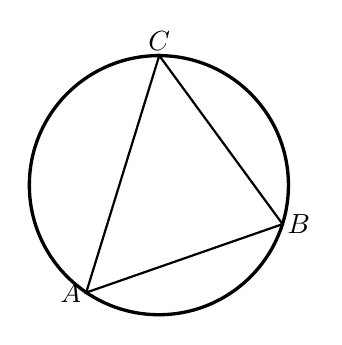
\begin{tikzpicture}
    \newcommand{\factor}{0.1}
    
    % basic triangle
    \pgfmathsetseed{100}
    \coordinate[label=left:$A$] (A) at (\factor*rand,\factor*rand);
    \coordinate[label=right:$B$] (B) at ($ (2.5,1) + \factor*(rand, rand) $);
    \coordinate[label=above:$C$] (C) at ($ (1,3.0) + \factor*(rand, rand) $);
    \draw (A) -- (B) -- (C) -- cycle;
    
    % draw middle orthogonal between #1 and #2 and name it #3
    \newcommand{\ortho}[3]{
        % p1 = orthogonal direction
        \begin{pgfinterruptboundingbox}
	        \path[name path global=#3] 
	             let \p1 = ($ #1!1.0!90:#2 - #1 $),
	                 \p2 = ($ #1!0.5!#2 $) 
	             in
    	             ($ (\p2) + 10.0*(\p1) $) -- ($ (\p2) - 10.0*(\p1) $);
        \end{pgfinterruptboundingbox}
    }
    % computes the circumcircle centre of #1,#2,#3 and name it #4    
    \newcommand{\circumcentre}[4]{
        \ortho{#1}{#2}{t1}
        \ortho{#2}{#3}{t2}        
        \path [name intersections={of=t1 and t2, by=#4}];
    }
    
    % mid lines 
    \circumcentre{(A)}{(B)}{(C)}{centre};
    \node[draw,circle through=(A),very thick] (circle) at (centre) {};
  \end{tikzpicture}
\end{document}